


\section{Evaluation}
%\subsection{Generalization to novel scenarios}
In our experiments we seek to validate the system's generalization capability to 1) novel object physical parameters 2) real-world dynamics, and 3) robot hardware embodiment. In all following experiments, both in simulation and the real-world, we use the same model trained with simulation training ropes generated in Sec. \ref{sec:data_generation}. The cloth placing task is evaluated in simulation only and is discussed in Sec. \ref{sec:cloth_eval}

\begin{figure}[t]
    \centering
    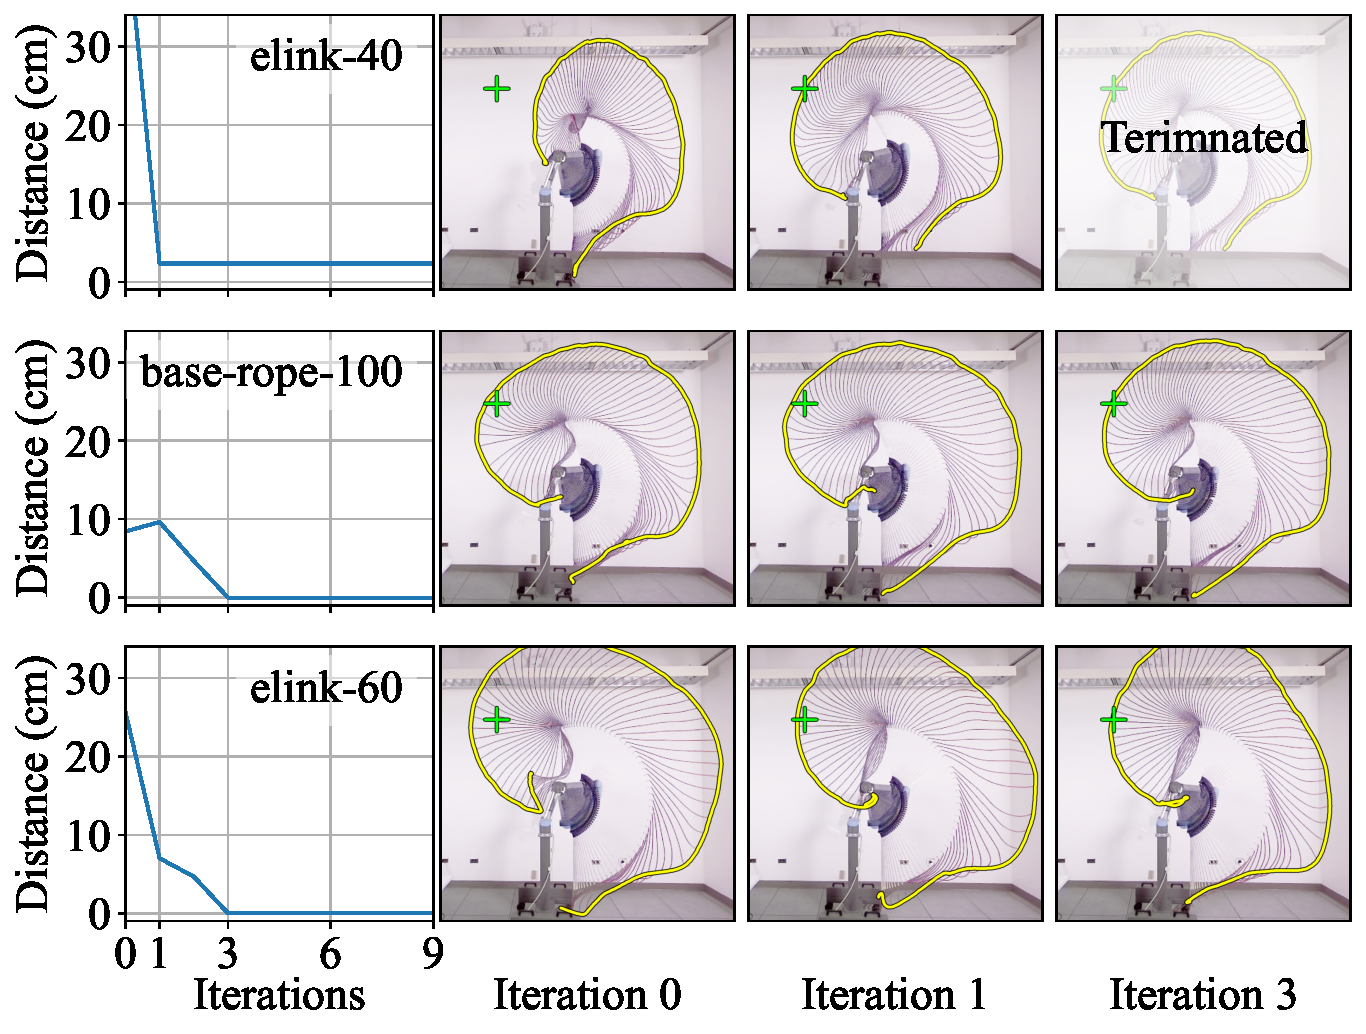
\includegraphics[width=\linewidth]{figure/elink_plot.pdf}
    \caption{\textbf{Adaptation to robot embodiment.}  We varies the robot's last link with 3 different lengths (40,50,60cm), which effectively changes the mapping between the actions and their effects. As expected, the robot with a different link than training (elink-40/-60) has a higher initial error. However, for all variations, the system is able to reach the goal by adjusting its action according to the visual feedback.} % \cheng{Note that the algorithm terminates once the distance is less than 2cm.}}
    %https://docs.google.com/drawings/d/1oiWSkWwh9zzMQ_cAMQME6a0cPVZw53zplIQvz1UpmLs/edit?usp=sharing
    \label{fig:real_stick} 
    \vspace{-6mm}
\end{figure}

\subsection{Rope Whipping Task}
\textbf{Metrics.}
We measure the performance of these algorithms using the minimum distance to the goal (in cm) at each step. The faster that an algorithm reaches a certain distance the better. We allow the maximum iteration to be 16 in simulation and 10 in real-world experiments. Note that the pixel size is around 2.3cm in our trajectory image encoding and the real-world tracking accuracy is around 1.3cm.

\textbf{Test Cases.}
To test the system's ability to generalize to different rope parameters, we used the following testing ropes: 
\begin{itemize}[leftmargin=*]
    \item Simulated ropes with parameters in the \textbf{interpolation} regime relative to the training rope parameters (Fig. \ref{fig:sim} green).
    \item Simulated ropes with parameters in the \textbf{extrapolation} regime relative to the training rope parameters (Fig. \ref{fig:sim} blue).
    \item \textbf{Real-world ropes} with different material, length, and mass distribution (Fig. \ref{fig:testcase} C). We modeled the simulation rope after the [base-rope], therefore all other ropes  are significantly out-of-distribution. In particular, the [bullwhip], and [knotted-rope] have a non-uniform mass distribution and the [long-cloth] has a larger surface area to density ratio, hence, experiences much larger aerodynamic effects (unmodeled in simulation) than to other ropes.     
\end{itemize}

\textbf{Robot hardware embodiment.} We validate the system's generalization capability to different robot hardware embodiments by sampling the robot's last link length from 3 different lengths, [elink-x] where x = 40cm,50cm,60cm. By changing robot's last link, we are effectively changing the mapping between the robot's action parameter and its physical embodiment, which require the system to adapt according to the new trajectory observations. Fig. \ref{fig:real_stick} shows the example results for this experiment, where \names~ converges to 3 different actions for the same goal.
% robot's action properties







\begin{table}[t]
\centering
    \setlength\tabcolsep{4pt}    
    \begin{tabular}{l|rrrrrr}
    \toprule
    {} &  OptSim &  AVG &  il-3 &  il-9 &  IRP-3 &  IRP-9 \\
    rope          &         &      &       &       &        &        \\
    \midrule
    base-rope-100 &    21.6 & 15.6 &  31.5 &  13.4 &    3.2 &    \textbf{1.3} \\
    base-rope-120 &    14.4 & 16.5 &  51.9 &  22.5 &    \textbf{1.9} &    \textbf{1.9} \\
    base-rope-60  &    14.5 & 19.9 &  28.4 &  28.0 &    8.9 &    \textbf{5.5} \\
    knotted       &    14.2 &  8.3 &  17.1 &   9.2 &    \textbf{2.6} &    \textbf{2.6} \\
    thick-rope    &    11.9 & 19.7 &  29.2 &  10.7 &   11.7 &    \textbf{3.2} \\
    long-cloth    &    15.8 & 59.6 &  72.2 &  16.8 &   14.0 &    \textbf{1.9} \\
    bullwhip      &    17.0 & 28.7 &  50.5 &   8.4 &    9.0 &    \textbf{1.9} \\
    \midrule
    elink-40      &    16.0 & 28.4 &  77.5 &  29.3 &   13.3 &    \textbf{6.1} \\
    elink-60      &    11.9 & 14.6 &  30.5 &  18.5 &    5.4 &    \textbf{3.8} \\
    \bottomrule
    \end{tabular}

    \caption{\textbf{Realworld Evaluation.} Distance to goal in cm for 7 unseen real world ropes and 2 robot hardware embodiments. [long-cloth] and [bullwhip] are particularly out-of-distribution. Our method significantly outperforms the other approaches we evaluated, demonstrating surprisingly strong generalization to unseen rope parameters, action definitions and simulation/reality divergence. IL: iterLinear. X-3, X-9 error measured in iteration 3 and 9.} \vspace{-4mm}
    \label{tab:real_eval} 
\end{table}



\textbf{Algorithm comparisons.} 
To validate the major design decisions and their impacts on performance, we compare with following alternative approaches: 
\begin{itemize}[leftmargin=3mm]
    \item \textbf{System identification (SysID, SysID\_GT)}:  This method first identifies key system parameters and then infers the action using these parameters. We give this baseline a head start by providing the true varying parameters in simulation: length and density. To ensure fairness, we use 16 fixed system identification actions to collect observations. Another 4-layer MLP is trained to regress the optimal action from estimated rope parameters. [SysID\_GT] is a variant of this baseline, where we assume the ground truth rope parameters are given.
    
    \item \textbf{Iterative control with heuristic (iterHeuristic):} A heuristic strategy that increases both the speed and amplitude of the action if the trajectory intersects with the line segment between the goal and the origin (the goal is outside the trajectory) and decreases otherwise. If the trajectory does not intersect with the ray from the origin to the goal, the algorithm terminates to prevent increasing error.
    % goal is in between the trajectory and the origin
    
    \item \textbf{Iterative control with linear model [iterLinear]}: 
    Instead of leveraging the residual dynamics model learned from offline data, a linear model of the plant is fitted on the trajectories observed so far, updated at each step. The action is adjusted at each step by minimizing the shortest distance to the goal using the linear model.
    
    \item \textbf{Direct delta action regression [DeltaReg].} Instead of using sampled delta actions as input, this method directly regresses the optimal delta action for the goal and the observed trajectory. The model is trained with MSE loss.  We test it with the same number of iterations.
    
    \item \textbf{No adaptive action sampling [ConstSigma].} An ablation of our method which uses a fixed sigma for action sampling.
    
    \item \textbf{Average action in simulation (AVG):} The action that minimizes the average distance to goal in the training set, regardless of rope parameters, this is also the action we used to initialize our method at step one. 
    
    \item \textbf{Optimal control in simulation (OptSim):} This method estimates optimal actions in simulation with measured rope parameters from a real-world (i.e., length, density and width). This method represents an oracle for model-based control using our simulator. It is used only in real-world experiments to quantify the sim2real gap.
\end{itemize}

\begin{figure}[t]
    \centering
    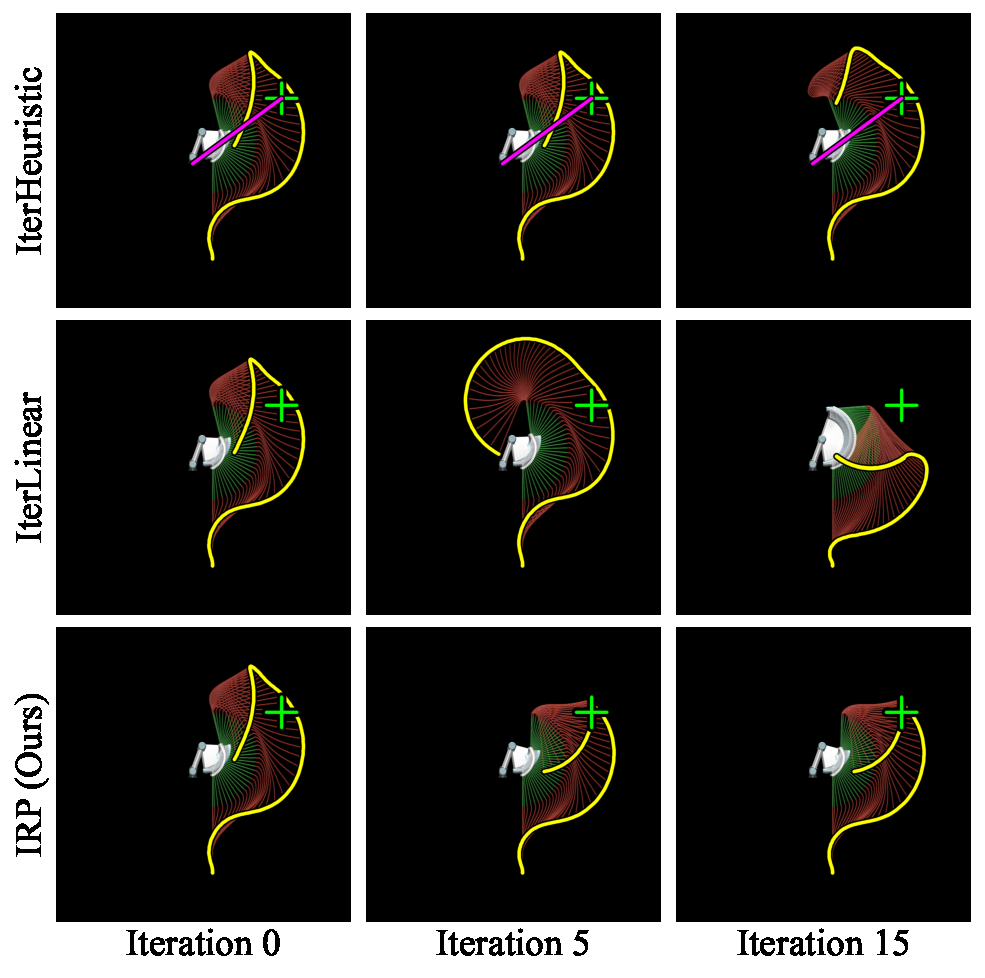
\includegraphics[width=\linewidth]{figure/heuristic_compare_plot.pdf}
    \caption{\textbf{Comparison.} In this example, the rope trajectory switches between several discrete modes. As a result, IterHeuristic gets stuck in a sub-optimal orbit and iterLinear failed to approximate the switching behavior. In contrast, our method accurately predicts the switching behavior and reaches the goal.} \vspace{-4mm}
    %  
    \label{fig:comparison}
    \vspace{-3mm}
\end{figure}

\subsection{Experimental Analysis}
\textbf{Benefits of learning residual dynamics.} 
% One of the key features of our method is learning the residual trajectory based on an observed trajectory instead of the entire dynamical process. 

We hypothesize that this formulation eases the learning process and maintains the flexibility of representing complex non-linear dynamics. To validate this hypothesis, we compared to other alternatives for modeling the system.


%\cheng{One of the key ideas of our method is to only capture small changes in trajectory given changes in action, instead of predicting the entire dynamical process from scratch. We hypothesize that this formulation eases the learning process and still be flexible in representing complex dynamical system without sacrificing expressibility.To validate the effectiveness of the learned model to guide policy optimization, we compared to other alternatives for modeling the system.}

% One of the key ideas of our method is to learn the residual trajectory that captures the rope dynamics in a distributed and spatially localized fashion. We hypothesize that this formulation eases the learning process and still be flexible in representing complex dynamical system without sacrificing expressibility.
% To validate the effectiveness of the learned model to guide policy optimization, we compared to other alternatives for modeling the system.



Compared to the system identification method [SysID, SySId\_GT], \names~can better handle unmodeled physical parameters presented in real-world ropes (e.g., aerodynamics or stiffness), which is captured in the input trajectory but not in the predefined system parameters (e.g., length and density). As a result, the algorithm can adapt to real-world ropes much better than SysID methods. 
%This experiment demonstrates the importance of iterative online adaptation for closing the sim2real gap.
% As a result, the algorithm is able to adpat to significantly out-of-distribution ropes.


Compared to [DeltaReg], \names~ better models the multi-modal aspect of the solution space.
Oftentimes there are multiple actions could reach the same goal, where [DeltaReg] tends to predict the mean of all valid solution (due to its MSE objective), which is likely to be an invalid solution. 

%Since [DeltaReg] is trained on brute-forced optimal actions in the training set with MSE loss, it tends to predict the mean of multiple optimal actions, which is likely not a good solution itself.

% Compared to [DeltaReg], \names~is able to avoid regression to the mean problem. Since oftentimes there are multiple delta actions could reach the same goal, where the MSE loss tends to predict the mean of all valid delta actions, which might not correspond to any valid solution. 

Compared to [IterHeuristic], our learned \names~model can capture complexity in the rope dynamics, such as mode switching when crossing key velocity thresholds, that the heuristic approach cannot capture. The [IterHeuristic] policy essentially assumes that the tip of the rope swings in a full circle, with its radius controlled by the action's energy. However, when the energy is insufficient for the tip to swing past apex this assumption is incorrect, and therefore, lead to incorrect action prediction. 
Moreover, around the apex point, the rope trajectory quickly switches between several modes, causing [IterHeuristic] to get stuck in oscillating local minima (Fig. \ref{fig:comparison} first row).
%Moreover, the step size gain of this heuristic method also needs to be carefully tuned to prevent the algorithm from diverging.
% It is especially true when the action is close to the limit, or the rope trajectory is changing between distinct modes (Fig. \ref{fig:comparison} first row). In these cases, the heuristic policy often moves in the incorrect direction, or causes little change to the trajectory, resulting in poor performance.  Moreover, the step size gain of this heuristic method also needs to be carefully tuned to prevent the algorithm from diverging. 

Finally, compared to [iterLinear]: our \names~model is able to converge in fewer steps with lower distance. In many cases, the rope trajectories switch between several discrete modes for different actions in a highly non-linear fashion, which cannot be easily captured by the linear model (Fig. \ref{fig:comparison}  second row). In contrast, our model is able to learn a non-linear model from the diverse set of training trajectories. 


\begin{figure}[t]
    \centering
    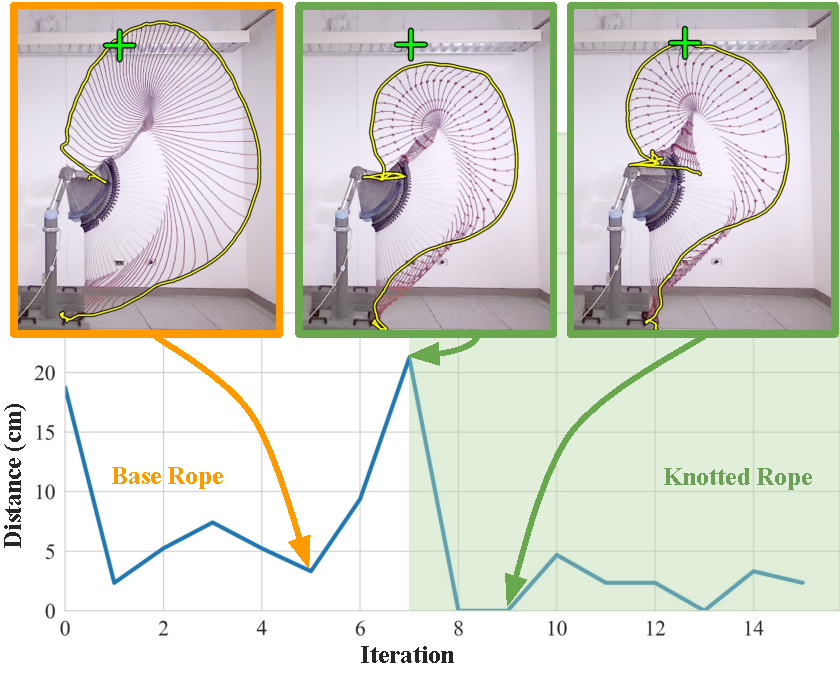
\includegraphics[width=\linewidth]{figure/rope-interrupt_plot.pdf}
    \caption{\textbf{Online adaptation to system  changes.} In this experiment, the robot first interacts with  [base-rope-100]. At step 6, the rope is knotted. We plot the distance to goal with respect to the steps.  While the tied knots significantly change the rope's length, density and mass distribution, the system is able to quickly adjust to the new system dynamics and achieve low errors.}
    \label{fig:online_adaptation} \vspace{-4mm}
    % https://docs.google.com/drawings/d/1FruOFXWzqVgBtRp5RsSdP1RR39_toRoPP4JaDZYy74U/edit?usp=sharing
\end{figure}
 
\begin{figure*}[t]
    \centering
    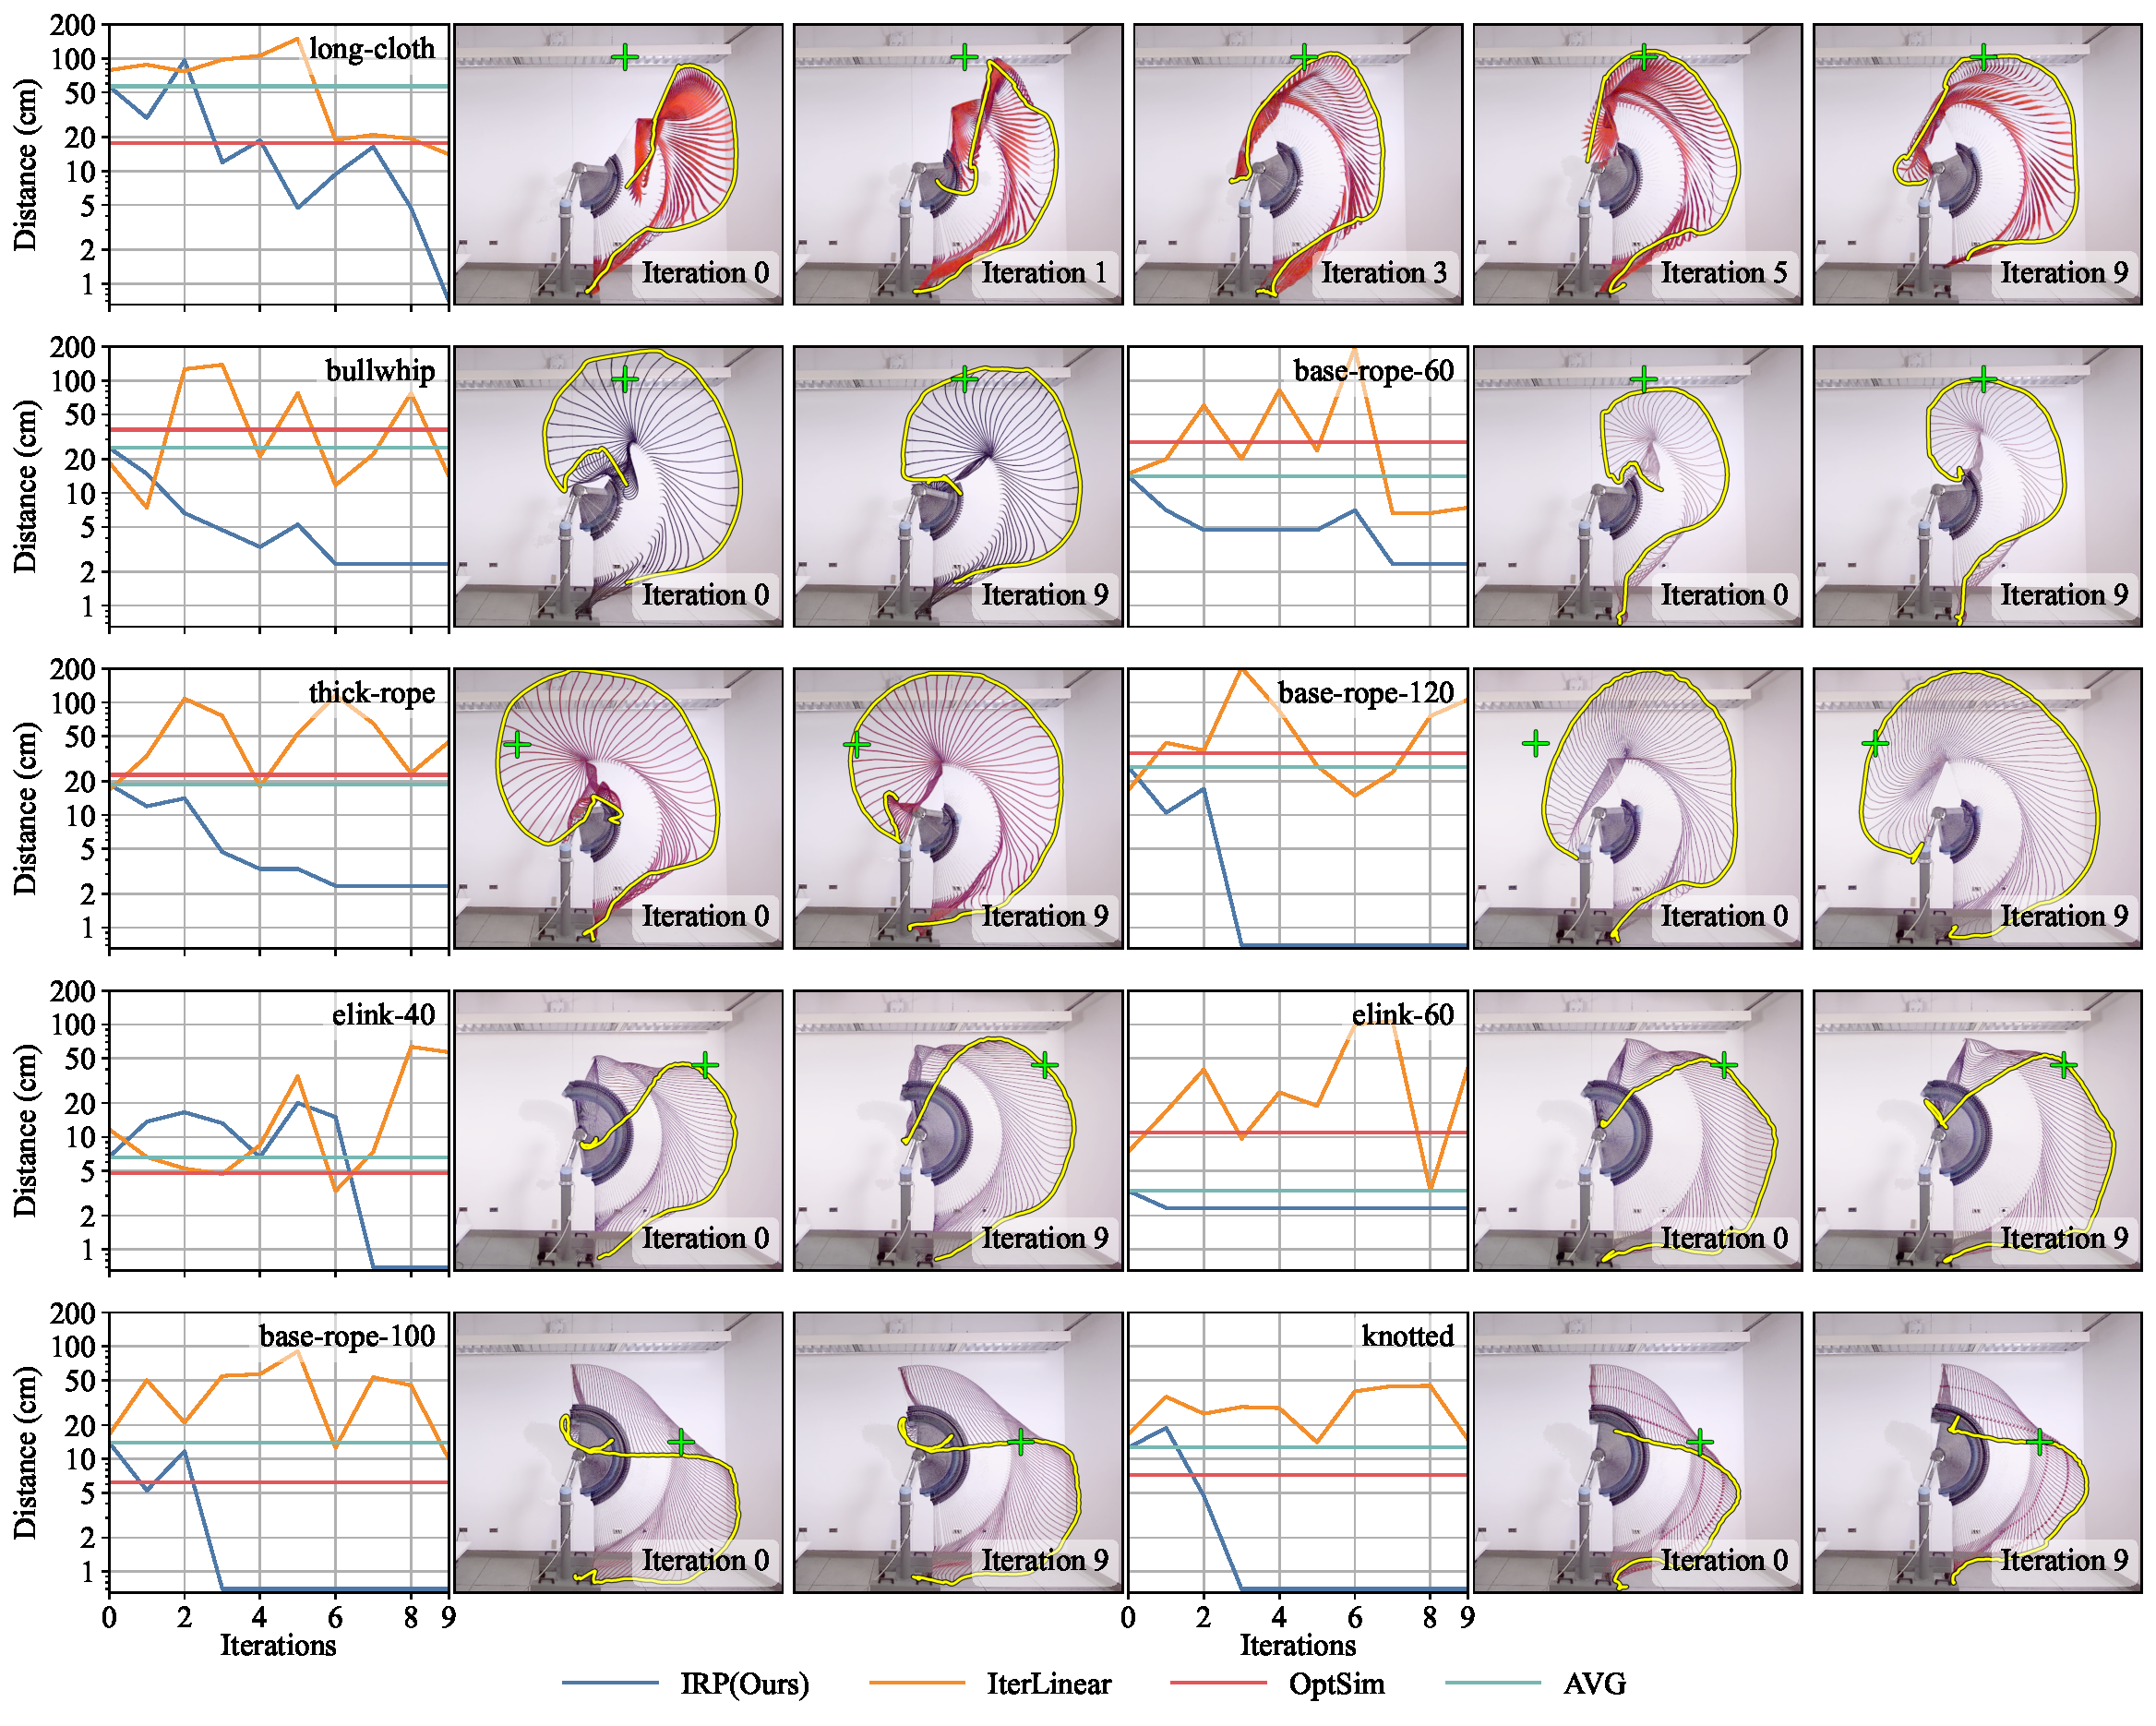
\includegraphics[width=\linewidth]{figure/real_vis_plots.pdf} 
    \vspace{-6mm}
    \caption{\textbf{Real-world test results on different ropes.} Using the same network trained on simulation data only, our method is able to generalize to significantly out-of-distribution ropes and a wide range of goals. First row: step 0,1,3,5 and 9 for long-cloth test case. Second row: step 0, 9 for other test cases. OptSim is not able to achieve low error, indicating the large sim2real gap in this task. All distances are shown in \textbf{log scale}. iterLinear failed to find good solutions within 9 steps, since it uses online observations only and has limited model capacity. More results can be find in the supplemental video.} 
    %https://docs.google.com/drawings/d/1qIPaECj8m26UyuAT7611URPWJPjAzNO1Q7S1zr13SZE/edit?usp=sharing
    \vspace{-4mm}
    \label{fig:real_detail}
\end{figure*}
\textbf{Benefits of iterative action refinements.}
With its iterative refinements, \names~can consistently improve its performance from the best average action.  On average, the error drops 94\% on interpolation experiments and 91\% drop on extrapolation experiments by using the additional trajectory observations. 
%This result demonstrates that \names~is able to consistently improve its action estimation based on additional observations of the rope trajectories.
Moreover, the comparison with [ConstSigma] shows that the adaptive action sampling method (described in Sec. \ref{sec:method_sample}) can further improve the action samples and prevent overshooting around the optimal action --- demonstrated by higher error and variance for [ConstSigma] in Fig. \ref{fig:sim} C after step 4. 

\textbf{Comparison to optimal control in simulation.}
By computing the action using exhaustive search with manually measured parameters, the performance of [OptSim] represents an \textit{oracle} for trajectory optimization using our MuJoCo simulation environment, and it should achieve perfect result in the simulated environments.  
However, due to the instability of the dynamical system and unmodeled effects such as aerodynamics, [OptSim] still results in higher error compared to \names~in our real-world experiment (Fig \ref{fig:real_detail}, Tab. \ref{tab:real_eval}). 
This result demonstrates the importance of online adaptation for closing sim2real gaps, especially for complex dynamical systems such as the dynamic manipulation of deformable objects.
%These results demonstrates that both the  and the iterative action refinement are the key enabler for the success sim2real adaptation.  

\textbf{Online adaptation to system changes.}
In this experiment, we stress test \names' robustness against unexpected system changes during the interaction steps. We first ask the robot to interact with the [base-rope-100]. After step 6, we tie four knots on the rope and observe the system behavior.  While the tied knots significantly changes the rope's length, density and mass distribution, we observe that the system is able to quickly adjust to the new system dynamics and regain good performance ( Fig. \ref{fig:online_adaptation}). 


\section{Extension to Cloth Manipulation}
\label{sec:cloth_eval}
To demonstrate the generality of \names's, we applied the same method to a cloth placement task with minimal modifications.

\textbf{Test cases.}
We randomly sampled five unseen cloth parameter pairs (size, density) as our testing cases. For each cloth sample, we uniformly sampled 11 goal configurations from the range illustrated in Fig. \ref{fig:cloth_plot} A. Note that since test cloths all have different sizes, the specific target keypoint locations are adjusted accordingly. 

\textbf{Metrics.}
The performance is measured by the average distance to the goal (in cm) over all keypoints. Note that due to the stretching effects on the cloth and the thickness of MuJoCo's capsule model for collision, it is not possible to reach zero error for a target configuration with perfectly square and flat keypoint locations.

\textbf{Result.}
Fig \ref{fig:cloth_plot} B and C show the qualitative and quantitative results respectively. Fig \ref{fig:cloth_plot} B shows that \names~can adjust the action to different landing locations and shape of the cloth (e.g. to avoid folding). We compared with [DeltaReg] and [IterHeuristic], two of the best performing baseline methods from the rope whipping task. We modified the [IterHeuristic] to increase all action parameters if the landing keypoints are closer than the goal, and decreases otherwise, with the proportional gain set to $0.5$. On average, \names~achieves 3.5 cm error across 11 test goal configurations, yielding better performance and lower variance comparing to other methods.

\section{Conclusion}
This paper presents a general learning framework for goal-conditioned dynamic manipulation: \namel.  Our extensive experiments in both simulation and the real-world demonstrate its adaptability to many aspects of the system, including object parameters, real-world dynamics, and even robot hardware embodiment.
However, our method is not without limitations, one of which is the assumption of action repeatability, which can not be guaranteed in many applications.  We also assume full observability of the manipuland throughout the trajectory, which makes direct application of this approach difficult in highly cluttered scenarios.
Future work could explore using different visual feedback \cite{lin2021VCD,chi2021garmentnets} to deal with non-repeatable action scenarios and perception techniques leveraging temporal cues to handle partial observability \cite{xu2020learning}.



% \begin{table}[t]
%     \centering
%     \begin{tabular}{p{0.2\linewidth} | p{0.8\linewidth}}
%     \toprule
%      Names & Property \\
%      \midrule
%      base-rope-x  & Thin cotton ropes (13g/m) in 3 different lengths (x = 60cm, 100cm, 120cm).  \\
%      thick-rope   & A thick cotton rope (65g/m, 1m in length) \\
%      knotted & The base-rope-125 knotted with 3 knots \\ 
%      bullwhip & a leather whip with none-uniform mass distribution (average density 72g/m, 1m in length) \\
%      long-cloth & A piece of red cloth (1m in length 35mm in width, average density 19g/m)  \\
%      \midrule 
%      elink-x & Robot's last link (i.e., a wooden stick)  in 3 different lengths (x = 40cm,50cm,60cm)\\
%      \bottomrule
%     \end{tabular}
%     \caption{Realworld rope and their properties}
%     \label{tab:real_ropes}
% \end{table}

